\subsection{Klassifizierung der Verfahren zur Roboterprogrammierung}
\begin{figure}[ht]\centering 
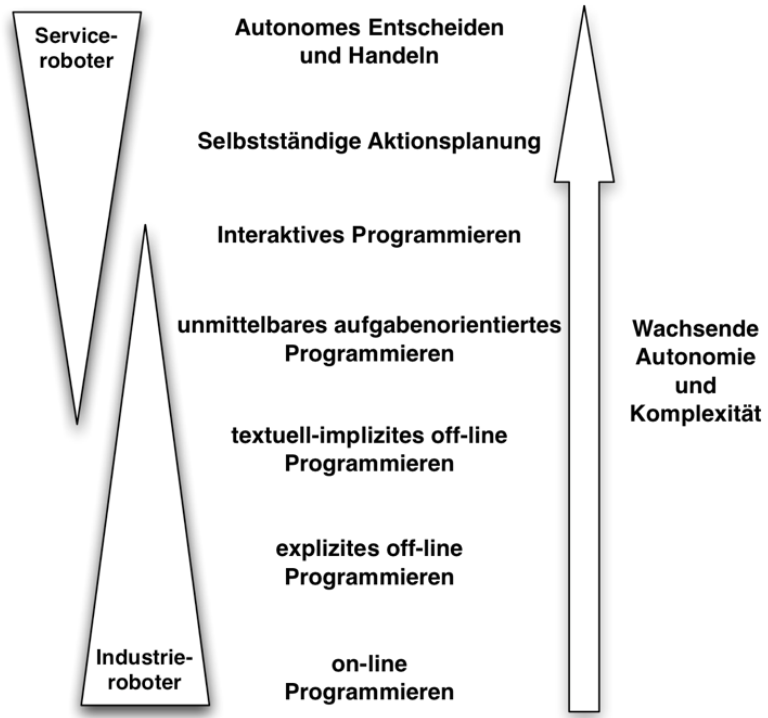
\includegraphics[width=0.5\linewidth]{figures/ch01_ueberblick.png}
\caption{Überblick}
\label{fig:ch01_komp}
\end{figure}
Kriterien:
\begin{itemize}
\item[1.] \textbf{Programmierort:} On-line (prozessnah, am Roboter) vs. Off-line (prozessfern, ohne Roboter)
\item[2.] \textbf{Art der Programmierung:} Direkte vs. indirekte (textuelle oder graphische/gemischte) Programmierung, hybride Verfahren
\item[3.] \textbf{Abstraktionsgrad der Programmierung:} Explizite/bewegungs- bzw. roboterorientierte vs. implizite/aufgabenorientierte Programmierung
\end{itemize}
\begin{figure}[ht]\centering 
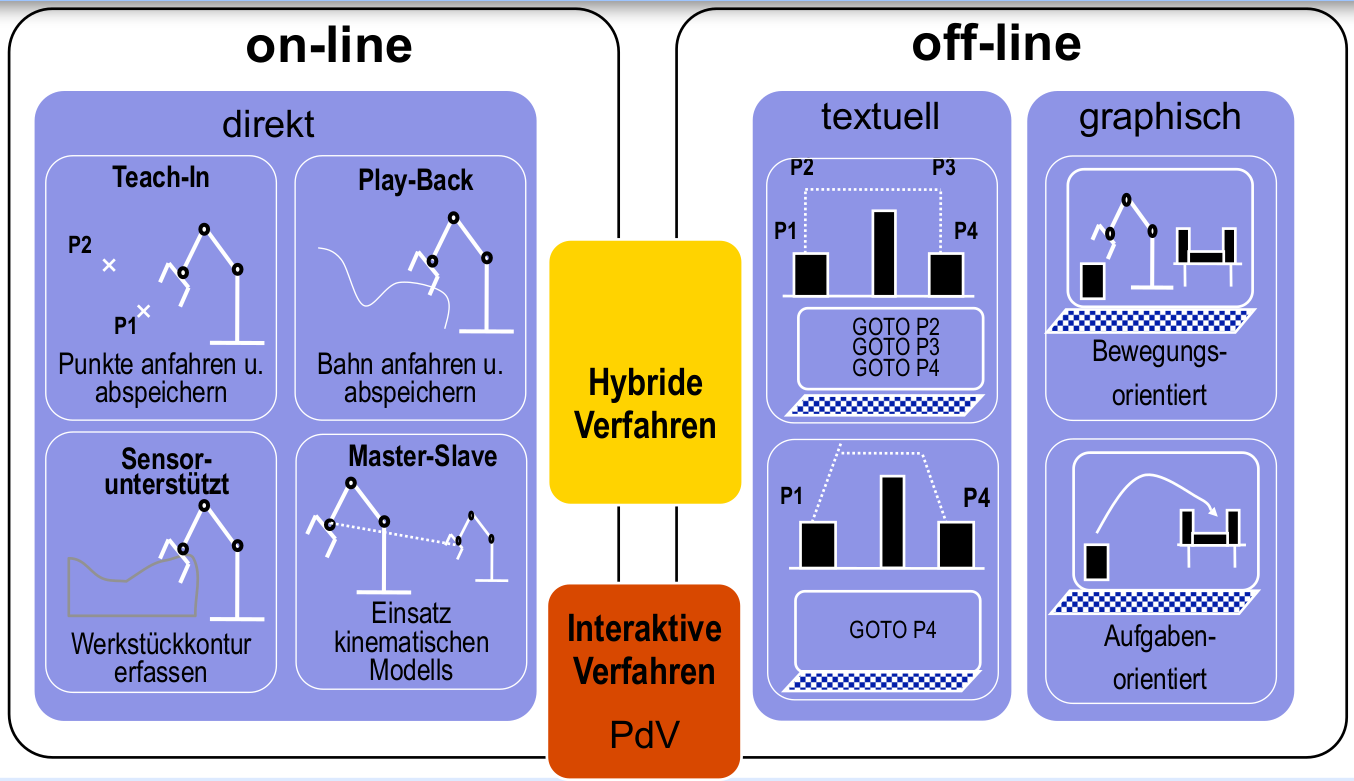
\includegraphics[width=\linewidth]{figures/ch01_schema.png}
\caption{Schema}
\label{fig:ch01_schema}
\end{figure}
\subsection{Arten der Programmierung}
\subsubsection{Direkte/Prozessnahe Programmierung}
\begin{itemize}
\item \textbf{Einstellen des Roboters:} Ältestes Programmierverfahren.
Der Bewegungsbereich jedes Gelenks wird durch Stopper eingeschränkt.
Die Bewegungen erfolgen für jedes Gelenk einzeln bis zum Anschlag.
Zuordnung zwischen Anfahrpunkten zu Stopper kann mit Codiermatritzen erfolgen.
(sogenannter \glqq Bang-Bang-Robot\grqq)\\
Nachteil: sehr kleine Menge von Anfahrpunkten.
\item \textbf{Teach-In Programmierung:} Anfahren markanter Punkte der Bahn mit manueller Steuerung
(Teach Box, Teach Panel, weitere: Spacemouse, Teach-Kugel)\\
Funktionalität einer Teach Box:
\begin{itemize}
\item Einzelbewegung der Gelenke
\item Bewegung des Effektors in 6 Freiheitsgraden
\item Punkte anfahren u. abspeichern
\item Speichern / Löschen von Anfahrpunkten
\item Eingabe von Geschwindigkeiten
\item Eingabe von Befehlen zur Bedienung des Greifers
\item Starten / Stoppen ganzer Programme
\end{itemize}
Vorgehensweise beim Teach-In:
\begin{itemize}
\item Anfahren markanter Punkte der Bahn (= Folge von Zwischenpunkten)
\item Speichern der Gelenkwerte
\item Ergänzung der gespeicherten Werte
um Parameter wie Geschwindigkeit, Beschleunigung usw.
\item Anwendung: in der Fertigungsindustrie (Punktschweißen, Nieten), Handhabungsaufgaben (Pakete vom Fließband nehmen)
\end{itemize}
\item \textbf{Play-Back- (manuelle) Programmierung:}
\begin{itemize}
\item Einstellung des Roboters auf Zero-Force-Control
(Roboter kann durch den Bediener bewegt werden)
\item Abfahren der gewünschten Bahn
\item Speichern der Gelenkwerte: automatisch (definierte Abtastfrequenz) oder manuell (durch Tastendruck)
\item Anwendung: mathematisch schwer beschreibbare Bewegungsabläufe, Integrierung der handwerklichen Erfahrung, typischerweise für Lackieren oder Kleben eingesetzt
\end{itemize}
\begin{table}[hbt]
\centering
\begin{tabular}{|p{13cm}|}
\hline
Nachteile\\
\hline
\vspace{-5mm}
\begin{itemize}
\setlength\itemsep{0em}
\item[-] schwere Roboter schwierig zu bewegen
\item[-] wenig Platz in engen Fertigungszellen für Bediener, dadurch Sicherheitsrisiko
\item[-] hoher Speicherbedarf (bei hoher Abtastrate)
\item[-] schlechte Korrekturmöglichkeiten
\end{itemize}\\
\hline
\end{tabular}
\caption{Nachteile der Play-Back-Programmierung}
\label{tab:PBprog}
\end{table}
\item \textbf{Master-Slave-Programmierung:}
\begin{itemize}
\item Bediener führt einen kleinen, leicht bewegbaren Master
Roboter (entspricht einem kinematischen Modell des
Slave-Roboters)
\item Bewegung wird auf den Slave-Roboter übertragen
\item Bewegungen werden synchron ausgeführt
\item Slave-Roboter wirkt als Kraftverstärker
\item Anwendung: Handhabung großer Lasten bzw. großer Roboter
\end{itemize}
\begin{table}[hbt]
\centering
\begin{tabular}{|p{6.5cm}|p{6.5cm}|}
\hline
Vorteile & Nachteile\\
\hline
\vspace{-5mm}
\begin{itemize}
\setlength\itemsep{0em}
\item[+] Möglichkeit, auch schwerste Roboter zu programmieren
\end{itemize}
 &
 \vspace{-5mm}
\begin{itemize}
\setlength\itemsep{0em}
\item[-] teuer, da zwei Roboter benötigt werden
\end{itemize}\\
\hline
\end{tabular}
\caption{Zusammenfassung Master-Slave-Programmierung}
\label{tab:MSprog}
\end{table}
\item \textbf{Sensorunterstützte Programmierung:}\\
Manuell
\begin{itemize}
\item Bediener führt Programmiergriffel (Leuchtstift, Laserstift) entlang der
abzufahrenden Bahn
\item Erfassung der Bewegung durch externe Sensoren (zB. Kameras,
Laserscanner)
\item Berechnung der inversen Kinematik
\end{itemize}
Automatisch
\begin{itemize}
\item Vorgabe des Start- und Zielpunktes
\item Sensorische Ertastung der Sollkontur (zB. über Kraft-Momenten-Sensor)
\end{itemize}
Anwendung: Abspeichern der Bahn als Folge der Gelenkwinkel
Schleifen, Entgraten von Werkstücken	
\end{itemize}
\begin{table}[hbt]
\centering
\begin{tabular}{|p{7.5cm}|p{7.5cm}|}
\hline
Vorteile & Nachteile\\
\hline
\vspace{-5mm}
\begin{itemize}
\setlength\itemsep{0em}
\item[+] schnell bei einfachen Trajektorien
\item[+] sofort anwendbar
\item[+] geringe Fehleranfälligkeit
\item[+] Bediener benötigt keine Programmierkenntnisse
\item[+] kein Modell der Umwelt erforderlich
\end{itemize}
 &
 \vspace{-5mm}
\begin{itemize}
\setlength\itemsep{0em}
\item[-] hoher Aufwand bei komplexen Trajektorien
\item[-] nur mit und am Roboter möglich
\item[-] spezifisch für einen Robotertyp
\item[-] Verletzungsgefahr durch Roboter
\end{itemize}\\
\hline
\end{tabular}
\caption{Zusammenfassung Direkte Programmierung}
\label{tab:dirprog}
\end{table}
\subsubsection{Textuelle Verfahren}
Erstellung von Robotersteuerprogrammen erfolgt mittels erweiterter,
höherer Programmiersprachen (PasRo, Val, etc.)
\\ \\
\textbf{Sprache:} (DIN 66025)
\begin{itemize}
\item Programm = Menge numerierter Sätze\\
z.B. \glqq N70 G00 X20 Z12\grqq{} entspricht Werkzeug im Eilgang (G00) an Position X=20 Z=12 bewegen. (N = Satznummer)
\item Sprachen:
\begin{itemize}
\item APT (Automatically Programmed Tools), 1961 MIT
\item EXAPT (Extended Subset of APT), 1966 Aachen
\end{itemize}
\end{itemize}

\begin{table}[!h]
\centering
\begin{tabular}{|p{7.5cm}|p{7.5cm}|}
\hline
Vorteile & Nachteile\\
\hline
\vspace{-5mm}
\begin{itemize}
\setlength\itemsep{0em}
\item[+] Programmierung kann unabhängig vom Roboter erfolgen
\item[+] strukturierte, übersichtliche Programmierlogik
\item[+] Erstellung komplexer Programme (Einbezug von Wissensbasis,
Weltmodell, Auswertung von Sensoren)
\end{itemize}
 &
 \vspace{-5mm}
\begin{itemize}
\setlength\itemsep{0em}
\item[-] Bediener benötigt Programmierkenntnisse
\item[-] keine / schlechte Korrekturmöglichkeiten
\end{itemize}\\
\hline
\end{tabular}
\caption{Zusammenfassung Textuelle Verfahren}
\label{tab:textprog}
\end{table}
\subsubsection{Graphische/Gemischte Verfahren}
\begin{itemize}
\item Graphische Darstellung von Kontrollstrukturen (if/else, Schleifen,
Marken...)
\item Kopplung mit Visualisierungs-Tool und Simulations-Tool (z.B. RobCAD)
\item  Trajektorien durch Interpolation aus Stützpunkten, Freihandzeichnen,
analytisch
\item Operationen Icon- oder Menu-gesteuert
\item Simple graphische Programmierung, z.B. Lego Mindstorms:
Leicht verständliche, ikonische Programmierung aber beschränkte Möglichkeiten
\item Graphische Programmierung basierend auf sensorieller Erfassung der
Benutzervorführung: Simulation der Roboterprogramme
\end{itemize}
\begin{table}[hbt]
\centering
\begin{tabular}{|p{7.5cm}|p{7.5cm}|}
\hline
Vorteile & Nachteile\\
\hline
\vspace{-5mm}
\begin{itemize}
\setlength\itemsep{0em}
\item[+] Programmierer benötigt weniger Programmierkenntnisse
\item[+] einfache Programmierung, leichte Fehlererkennung
\item[+] schnelles Erstellen komplexer Programme (rapid prototyping)
\end{itemize}
 &
 \vspace{-5mm}
\begin{itemize}
\setlength\itemsep{0em}
\item[-] sensorielle Benutzererfassung noch zu ungenau
\item[-] Leistungsfähige Hardware für Signalanalyse, Modellierung, ...
\item[-] Komplexe Modelle benötigt
\item[-] 2D-Sicht des Anwenders
\end{itemize}\\
\hline
\end{tabular}
\caption{Zusammenfassung Graphische Verfahren}
\label{tab:textprog}
\end{table}

\subsection{Abstraktionsgrad der Programmierung}
\subsubsection{Explizite/Roboterorientierte Programmierung}
\textcolor{red}{\glqq Wie ist es zu tun?\grqq} \\
Bewegungen und Greiferbefehle sind direkt in eine Programmiersprache eingebunden.\\
Das Aufgabenmodell ist gegeben durch Anfangs- und Endzustand (z.B. Relationale Darstellung). Ein Beispiel ist in \autoref{cran} dargestellt.
\begin{figure}[h!]\centering 
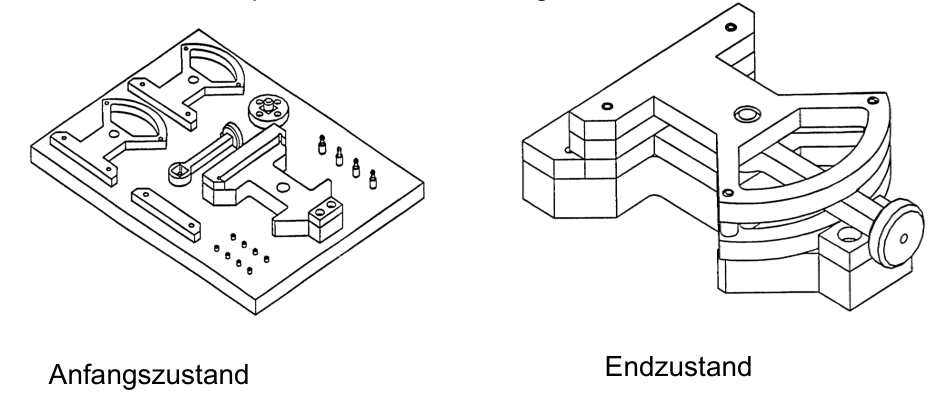
\includegraphics[width=0.7\linewidth]{figures/ch01_cranfield.png}
\caption{Der Cranfield-Montage-Benchmark}
\label{cran}
\end{figure}
\textbf{Anwender $\rightarrow$ Roboter}:\\
Jedes Robotersystem besitzt eine roboterabhängige Steuerungsebene, welche folgende Eigenschaften kapselt:
\begin{itemize}
\item Ansteuerung der Hardware (sowohl interne als auch externe)
\item Bewegungsaktionen
\item Lokale Modelle
\item Elementare Operationen (erfordern evtl. Echtzeitregelung)
\end{itemize}
\begin{figure}[h!]\centering 
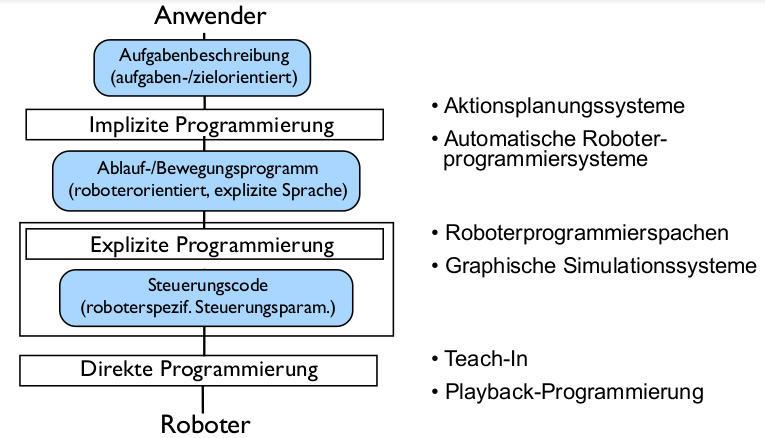
\includegraphics[width=0.7\linewidth]{figures/ch01_einordnung.png}
\caption{Einordnung roboterorientierten Programmierung}
\label{cran}
\end{figure}
\textbf{Anforderungen an die oboterorientierte Programmierung}:
\begin{itemize}
\item Positions-, Geschwindigkeitsregelung der aktiven Komponenten (z.B. Gelenke, Räder)
\item Auslesen und Parametrieren der internen und externen Sensorik
\item Koordinatentransformationen, direkte und inverse Kinematik
\item Sensorabhängige Regelung
\item Verfahren auf Trajektorien
\item Generierung und Zusammensetzen von Trajektorien zu komplexen Bewegungen
\item Verkettung komplexer Bewegungen zu Elementaroperationen
\end{itemize}
\textbf{Komponenten der roboterorientierten Programmierung}: \autoref{zykl}
\begin{figure}[h!]\centering 
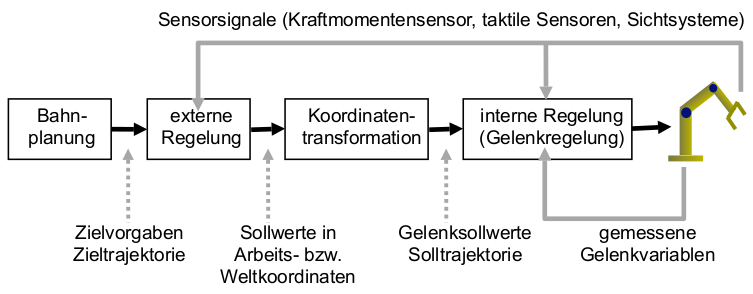
\includegraphics[width=0.7\linewidth]{figures/ch01_zykl.png}
\caption{Regelungszyklus eines Roboters}
\label{zykl}
\end{figure}
\textbf{Sprachelemente von Roboterprogrammiersprachen}:
\begin{itemize}
\item Befehle für:
\begin{itemize}
\item Bewegung eines oder mehrerer Roboter
\item Betrieb von Greifern / Werkzeugen
\item Ein-/Ausgabe von Daten / Signalen über Schnittstellen
\item Externe Sensoren
\item Zur Synchronisation / Kommunikation zwischen Prozessen
\item Parallelverarbeitung
\item Zur logischen Verkettung von Koordinatensystemen
\end{itemize}
\item Anweisungen zur Ablaufsteuerung
\item Definition generischer Operationen (zB. Armbewegung + Griff $\rightarrow$ ein Operator)
\end{itemize}
\textbf{Bewegungsanweisungen}:
\begin{itemize}
\item Bewegungen im Gelenkwinkelraum:
\begin{itemize}
\item Bewege alle Gelenke mit max. Geschwindigkeit
\item Regelung der Geschwindigkeiten mit gleichzeitiger Beendigung der Bewegung aller Gelenke
\end{itemize}
\item Kartesische Bewegungen (Stellung des TCPs)
\begin{itemize}
\item Erfordert inverse Kinematik
\item Nutzung von Frames, z.B. relativ zu einem Objekt
\end{itemize}
\item Geometriebezogene Bahndefinition
\end{itemize}
\begin{table}[hbt]
\centering
\begin{tabular}{|p{7.5cm}|p{7.5cm}|}
\hline
Vorteile & Nachteile\\
\hline
\vspace{-5mm}
\begin{itemize}
\setlength\itemsep{0em}
\item[+] Hohe Einstellgenauigkeit der Position
\item[+] Hohe Wiederholgenauigkeit
\item[+] eindeutige Roboterkonfiguration
\item[+] keine inverse Kinematik erforderlich
\end{itemize}
 &
 \vspace{-5mm}
\begin{itemize}
\setlength\itemsep{0em}
\item[-] Abhängigkeit von Robotertyp
\item[-] kein Bezug der Gelenkwinkel zur Objektlage
\end{itemize}\\
\hline
\end{tabular}
\caption{Bewegungen im Gelenkwinkelraum}
\label{tab:bew}
\end{table}
\textbf{Sprachelemente -- Semantik von Greiferbefehlen}
\begin{itemize}
\item Verschiedene Greifertypen: evtl. mit taktiler und/oder Kraftsensorik
\item Backengreifer: Industrie, Forschung (z.B. 3-Finger-Hand)
\end{itemize}
Mit zunehmender Abstraktion:
\begin{enumerate}
\item Steuerung im Gelenkwinkel-Raum
\begin{itemize}
\item Anzahl der Freiheitsgrade bestimmt Anzahl der Parameter (Backengreifer: 1, menschl. Hand: 22)
\item Wenig Kapselungs-Aufwand (keine inverse Kinematik nötig) 
\item Hand-abhängig
\item Kein Bezug zwischen Fingerstellung und Handstellung
\end{itemize}
\item Steuerung im kartesischen/ zylindrischen/... Raum
\begin{itemize}
\item Parameter: Position/Orientierung jedes Fingers/ jeder Fingerspitze
\item Inverse Kinematik nötig
\item Berechnung aus Greif-/ Bewegungsplanung oder aus menschlicher Vorführung
\item Mögliche Konfigurationen (Konfigurationsraum) handabhängig
\end{itemize}
\item Semantische Steuerung
\begin{itemize}
\item Parameter: Griff-Form, zu greifendes Objekt, Objektgröße, Objektform, ...
\item Mapping auf Roboterhand nötig
\item Übertragbar auf andere Roboterhände (mögliche Griffe handabhängig)
\item Griff-Form vom Menschen lernbar
\end{itemize}
\end{enumerate}
\textbf{Zusammenfassung -- Explizite Programmierung}: Nur in Verbindung mit (abstrakten) Programmiersprachen
\begin{table}[hbt]
\centering
\begin{tabular}{|p{7.5cm}|p{7.5cm}|}
\hline
Vorteile & Nachteile\\
\hline
\vspace{-5mm}
\begin{itemize}
\setlength\itemsep{0em}
\item[+] beliebig komplexe Bahnen
\item[+] Anbindung von Sensoren
\item[+] reaktive Planung
\end{itemize}
 &
 \vspace{-5mm}
\begin{itemize}
\setlength\itemsep{0em}
\item[-] Keine standardisierte Programmiersprache
\item[-] Kenntnis der Programmiersprache
\end{itemize}\\
\hline
\end{tabular}
\caption{Bewegungen im Gelenkwinkelraum}
\label{tab:bew}
\end{table}
\subsubsection{Implizite/Aufgabenorientierte Programmierung}
\textcolor{red}{\glqq Was ist zu tun?\grqq} \\
Die Aufgabe, die der Roboter durchführen soll, wird beschrieben, z.B. in Form von Zuständen.
\begin{itemize}
\item Abstrakte Form der Programmierung erfolgt in den Phasen\\
1. Modellierung der Umwelt\\
2. Spezifikation der Aufgaben\\
3. Erzeugung der Roboterprogramme
\item u. U. erfolgt vor der Ausführung eine Überprüfung des
Roboterprogramms (Simulation)
\item Beispiel: Einschenken unter Berücksichtigung von Hindernissen
\item Details im kommenden Kapitel
\end{itemize}